\documentclass{article}

% if you need to pass options to natbib, use, e.g.:
% \PassOptionsToPackage{numbers, compress}{natbib}
% before loading nips_2016
%
% to avoid loading the natbib package, add option nonatbib:
% \usepackage[nonatbib]{nips_2016}

\usepackage[final]{nips_2016}

% to compile a camera-ready version, add the [final] option, e.g.:
% \usepackage[final]{nips_2016}

\usepackage[utf8]{inputenc} % allow utf-8 input
\usepackage[T1]{fontenc}    % use 8-bit T1 fonts
\usepackage{hyperref}       % hyperlinks
\usepackage{url}            % simple URL typesetting
\usepackage{booktabs}       % professional-quality tables
\usepackage{amsfonts}       % blackboard math symbols
\usepackage{nicefrac}       % compact symbols for 1/2, etc.
\usepackage{microtype}      % microtypography
\usepackage{graphicx}
\usepackage{bm}
\usepackage{amsfonts,amssymb}
\usepackage{amsmath}
\usepackage[linesnumbered, ruled]{algorithm2e}
\usepackage{float}
 
\bibliographystyle{plain}

\title{Survey on Image Inpainting}

% The \author macro works with any number of authors. There are two
% commands used to separate the names and addresses of multiple
% authors: \And and \AND.
%
% Using \And between authors leaves it to LaTeX to determine where to
% break the lines. Using \AND forces a line break at that point. So,
% if LaTeX puts 3 of 4 authors names on the first line, and the last
% on the second line, try using \AND instead of \And before the third
% author name.

\author{
  Tianyuan Zhang \\%\thanks{Course project} \\
  Department of Computer Science\\
  Peking University\\
  \texttt{1600012888@pku.edu.cn} \\
  }
\usepackage{xcolor}
\newcommand\yx[1]{\textcolor{cyan}{[Yilun Xu: #1]}}
\begin{document}
% \nipsfinalcopy is no longer used

\maketitle

\begin{abstract}
  Crowdsourcing has become a popular paradigm for collecting labels of large-scale datasets. However, the collected labels are noisy out of the inaccuracy of experts,thus we need to aggregate labels to complete a supervised problem. Traditional methods often fail because the complexity and non-convexity of the log-likelihood function. In this paper, we suppose the experts are people with different ability and the each data point has unique difficulty. Then we tackle the problem via EM algorithm together with our original difficulty processing method. Furthermore, we show the superiority of our method through ablation study with synthesized data and real data.
\end{abstract}

\section{Introduction}
In this data-driven times, the need for large-scale data has become more urgent than any time in the history. Crowdsourcing come up to solve the problem under such background, eliciting labels from crowds to accomplish this mission cosmically. As the name suggests, most crowdsourcing services resort to labeling redundancy, collecting multiple labels from different workers for each item.  Though this solution seems appropriate, new problem emerges that the labeled data coming from crowds are always noisy out of non-consistency of workers' ability or the high difficulty of certain task like age estimation or medical images annotation. Under such scenario, several problems are raised:
\begin{itemize}
\item how to aggregate and infer the ground truth label from the noisy crowdsourced labels?
\item how to learn an accurate data classifier based on the imperfect crowdsourced labels?
\end{itemize}
Maybe the most naive way to solve this problem is \emph{Majority Vote}, which simply assigns the label returned by the majority of the workers and learning a data classifier with the majority answer. But biased answer can be obtained with a difficult task when most experts get wrong, causing it to be an error-prone algorithm.

Apart from majority vote, a classical method proposed by \cite{dawid1979maximum} develop  a maximum likelihood approach based on the EM algorithm. They assume that each worker is associated with a $2\times 2$ confusion matrix, where the (l,c)-th entry represents the probability that a random chosen item in class l is labeled as class c by the worker: 
\begin{displaymath}
\left( \begin{array}{cc}
\alpha & 1-\alpha \\
1-\beta & \beta  \\
\end{array} \right)
\end{displaymath}
Hereafter we denote $\alpha=\textup{Pr}[y^{\mathrm{worker}}=1|y=1]$ and $\beta=\textup{Pr}[y^{\mathrm{worker}}=0|y=0]$. The true labels and worker confusion matrices are jointly estimated by maximizing the likelihood of the observed labels, where the unobserved true labels are treated as latent variables.

From the path of \cite{dawid1979maximum}, our baseline \cite{raykar2010learning} improved the algorithm with a logistic regression classifier. Besides, it extends the confusion matrix' setting to a worker-independent one. A bayesian approach is also discussed.

Nevertheless, this method is also constrained and often fails for it assumes that the confusion matrix only depends on the specific worker and has nothing to do with data. In reality, however, there does exist data that is hard for people (worker) to deal with:

\begin{figure}[H]
    \centering
    
\includegraphics[width=3in]{image/MNIST_confused_example1.png}
    \caption{left \& middle: images that are hard to classify \quad right: image that is easy to classify} 
    \label{fig:MNIST_confused_example1}
\end{figure}

Thus assigning a measure of difficulty for each data is necessary. In our approach, we design two algorithm, named \textbf{Adaptive Difficulty EM} and \textbf{Fixed Difficulty EM}. Details can be seen in latter sections. Empirical studies show that our approach is more competent than our baseline in both synthesized and real dataset.

\section{Related Works}

A series of works consider crowdsourcing problem by mixing the learning process and the aggregation process together. \cite{karger2014budget} transorm the learning from crowds problem into a maximum likelihood estimation (MLE) problem, then implement an EM algorithm to jointly learn the expertise of different experts and the parameters of a logistic regression classifier. \cite{albarqouni2016aggnet} extend this method to combine with the deep learning model. \cite{khetan2017learning} also reduce the learning problem to MLE and assume that the optimal classifier gives the ground truth labels and the experts make independent mistakes conditioning on the ground truth. Unlike our method, these MLE based algorithms are not robust to correlated mistakes. Recently, \cite{guan2018said} and \cite{rodrigues2018deep} propose methods that model multiple experts individually and explicitly in a neural network. However, their works lack theoretical guarantees and are outperformed by our method in the experiments, especially in the naive majority case. Moreover, unlike our method, their methods cannot be used to employ both the data and the crowdsourced labels to forecast the ground truth. 

Another series of methods are based on the generative model proposed by \cite{dawid1979maximum}. In particular, \cite{ghosh2011moderates} propose a method based on Singular Value Decomposition (SVD) which addresses binary labeling problems under the one-coin model. The analysis in it assumes that the labeling matrix is full, that is, each worker labels all items. To relax this assumption, \cite{dalvi2013aggregating} propose another SVD-based algorithm which explicitly considers the sparsity of the labeling matrix in both algorithm design and theoretical analysis. It proposed an iterative algorithm for binary labeling problems under the one-coin model  and extended it to multi-class labeling tasks by converting a $k$-class problem into $k-1$ binary problems. This line of work assumes that tasks are assigned to workers according to a random regular graph, thus imposes specific constraints on the number of workers and the number of items. 

Several works focus on modeling the experts. \cite{whitehill2009whose} model both expert competence and image difficulty, but did not consider expert bias.
\cite{welinder2010multidimensional} model each expert as a multidimensional classifier in an abstract feature space and consider both the bias of the expert and the difficulty of the image. \cite{rodrigues2014gaussian} model the crowds by a Gaussian process. \cite{shah2016permutation} consider the generalized Dawid-Skene model \cite{dawid1979maximum} which involves the task difficulty. However, these works are still not robust to correlated mistakes.

\section{Our Approach}
\subsection{Traditional Two-coin Model}
Let $y$ be the actual but unobserved label for the instance and $y^{j} \in \lbrace 0,1 \rbrace$. Suppose each annotator has sensitivity $\alpha^{j}$ and specificity $\beta^{j}$. 

The sensitivity is defined as the probability that an expert labels a positive sample as one.$$\alpha^{j}:=\textup{Pr}[y^{j}=1|y=1]$$
The specificity is defined as the probability that an expert labels a negative sample as zero. $$\beta^{j}:=\textup{Pr}[y^{j}=0|y=0]$$
If we model the classification problem using logistic regression, that is,
$$\textup{Pr}[y=1|\bm{x},\bm{\omega}]=\sigma(\bm{\omega}^{T}\bm{x})$$
and we maximize the likelihood,
$$\textup{Pr}[\mathcal{D}|\bm{\theta}]=\prod^{N}_{i=1}\{\textup{Pr}[y_i^1,...,y_i^R|y_i=1,\bm{\alpha}]\textup{Pr}[y_i=1|\bm{x_i},\bm{w}]+$$
$$\textup{Pr}[y_i^1,...,y_i^R|y_i=0,\bm{\beta}]\textup{Pr}[y_i=0|\bm{x_i},\bm{w}]\}$$
where $\bm{\theta}=\{\bm{\alpha,\beta,\omega}\}$
The problem could be solved by EM algorithm.
\begin{itemize}
    \item \textbf{E-step}. Given $\{\bm{\alpha,\beta,\omega}\}$ we compute the posterior probability
    $$\mu_i = \frac{a_i p_i}{a_i p_i+b_i(1-p_i)}$$
    where we defined
    \begin{align*}
        &p_i:=\sigma(\bm{\omega^T}\bm{x_i})\\
        &a_i:=\prod^R_{j=1}[\alpha^j]^{y_i^j}[1-\alpha^j]^{1-y_i^j}]\\
        &b_i:=\prod^R_{j=1}[\beta^j]^{1-y_i^j}[1-\beta^j]^{y_i^j}
    \end{align*}
    \item \textbf{M-step}. We have closed form solution for $\bm{\alpha}$,$\bm{\beta}$.
    $$\alpha_j=\frac{\sum^N_{i=1}\mu_i y_i^j}{\sum^N_{i=1}\mu_i}, \quad \beta_j=\frac{\sum^N_{i=1}(1-\mu_i)(1-y_i^j)}{\sum^N_{i=1}(1-\mu_i)}$$
    For $\bm{\omega}$, we use the Newton-Raphson update given by $\bm{\omega}^{t+1}=\bm{\omega}^t-\eta\bm{H}^{-1}\bm{g}$,where
    \begin{align*}
        \bm{g(\omega)}&=\sum^N_{i=1}[\mu_i-\bm{sigma}(\bm{\omega^T\bm{x_i}})]\bm{x_i}\\
        \bm{H(\omega)}&=-\sum^N_{i=1}[\sigma(\bm{\omega^T x_i})][1-\bm{sigma}(\bm{\omega}^T\bm{x_i})]\bm{x_ix_i^T}
    \end{align*}
    
\end{itemize}
    

\subsection{Our Modification}
In the model above, we assume that every instance is the same for a certain expert, which is obviously unrealistic. We assume $\alpha$ is correlated with factors in two dimensions, the ability of an expert and the difficulty of a classification task. In addition, we assume the form of $\alpha_{i}^{j}$ and 
$\beta_{i}^{j}$ as
$$\alpha_{i}^{j}=\bm{\sigma}\lbrace\lambda_{j}^{1}(p_{i}-1/2)^{2}\rbrace$$
$$\beta_{i}^{j}=\bm{\sigma}\lbrace\lambda_{j}^{2}(p_{i}-1/2)^{2}\rbrace$$
where $\lambda_j^1$ and $\lambda_j^2$ are positive real numbers and $p_i=\textup{Pr}[y_i=1|x_i, \bm{\omega}]$, which is given by classifier. $\sigma(\cdot)$ denotes the sigmoid function

To make the structural assumption clear, we point out:
\begin{itemize}
    \item In terms of the instance, if $p_i$ is close to 1/2, which implies the instance is close to decision boundary and thus the instance might well be hard to classify.
    \item In terms of the expert, she might have different abilities dealing with positive instances and negative ones, which implies difference between  $\lambda_j^1$ and $\lambda_j^2$. For larger $\lambda^{1}$ and $\lambda^{2}$, the expert has higher possibility to do the right classification.
\end{itemize}

In the meanwhile, we train two types of classifiers, one is logistic regression as in the original paper, the other is neural network, which is believed to perform better in complex classification task.

\subsection{Learning Problem}
Given the training data $\mathcal{D}$ consisting of N instances with annotations from R annotators, the task is to estimate the classifier parameter $\bm{\omega}$, which can be used for future prediction, the sensitivity ability $\bm{\lambda^1}=[\lambda_1^1,\lambda_2^1,...,\lambda_R^1]$ and the specificity ability $\bm{\lambda^2}=[\lambda_1^2,\lambda_2^2,...,\lambda_R^2]$ of R experts, which can help evaluate these experts. The estimated ground truth $\lbrace y_1,...,y_N\rbrace$ is also of interest.

\subsection{Maximum Likelihood Estimator}
We introduce the parameters $\bm{\theta}=\lbrace \bm{\omega,\lambda}\rbrace$, where $\bm{\omega}$ is the parameters for the classifier, $\bm{\lambda=\lbrace\lambda^{1},\lambda^{2}}\rbrace$.

Assuming the training instances are independent, the likelihood function can be factored as $$\textup{Pr}[\mathcal{D}|\bm{\theta}]=\prod_{i=1}^{N}\textup{Pr}[y_i^1,...,y_i^R|\bm{x_i},\bm{\theta}]$$
Conditioning on the true label $y_i$ and let $p_i=\textup{Pr}[y_i=1|\bm{x_i},\bm{\omega}]$
$$\textup{Pr}[\mathcal{D}|\bm{\theta}]=\prod_{i=1}^{N}\lbrace \textup{Pr}[y_i^1, y_i^2,...,y_i^R|y_i=1,\bm{\lambda^1},p_i]\cdot p_i+ \textup{Pr}[y_i^1,y_i^2,...,y_i^R|y_i=0,\bm{\lambda^2},p_i]\cdot (1-p_i) \rbrace$$
Assuming experts make decisions independently
$$\textup{Pr}[\mathcal{D}|\bm{\theta}]=\prod_{i=1}^{N} \lbrace \prod_{j=1}^{R} \textup{Pr}[y_i^j|y_i=1,\lambda_j^1,p_i]\cdot p_i+\prod_{j=1}^{R}\textup{Pr}[y_i^j|y_i=0,\lambda_j^2,p_i]\cdot (1-p_i \}$$
The likelihood can be written as
$$\textup{Pr}[\mathcal{D}|\bm{\theta}]=\prod_{i=1}^{N}[a_i p_i+b_i (1-p_i)]$$
where we define
$$a_i:=\prod_{j=1}^R[\sigma\{ \lambda_j^1(p_i-1/2)^2 \}]^{y_i^j} [1-\sigma\{ \lambda_j^1 (p_i-1/2) \}]^{1-y_i^j} $$
$$b_i:=\prod_{j=1}^R[\sigma\{ \lambda_j^2(p_i-1/2)^2 \}]^{1-y_i^j} [1-\sigma\{ \lambda_j^2 (p_i-1/2) \}]^{y_i^j} $$
The maximum-likelihood estimator is found by maximizing the log-likelihood
$$\hat{\bm{\theta}}=\lbrace \bm{\hat{\omega},\hat{\lambda}}\}$$
\subsection{Adaptive Difficulty EM Algorithm}
We use the EM algorithm to compute the maximum likelihood solution. Suppose we know the missing ground truth $\bm{y}=[y_1,y_2,...,y_N]$, then the likelihood can be written as 
$$\textup{ln} \textup{Pr}[\mathcal{D},\bm{y}|\bm{\theta}]=\sum_{i=1}^N y_i \textup{ln}(p_ia_i)+(1-y_i)\textup{ln}(1-p_i)b_i$$
Each iteration consists of two steps: E-step and M-step.
\begin{itemize}
    \item \textbf{E-step}. Given $\mathcal{D}$ and current estimation of $\bm{\theta}$, we can compute posterior probability
    $$\mu_i=\textup{Pr}[y_i=1|y_i^1,...,y_i^R,\bm{x_i},\bm{\theta]}=\frac{a_ip_i}{a_ip_i+b_i(1-p_i)}$$
    \item \textbf{M-step}. Given $\mu$, we can maximize the lower bound on the true likelihood,
    $$\textbf{\textup{E}}\{\textup{ln}\textup{Pr}[\mathcal{D},
    \bm{y}|\bm{\theta}]\}=\sum_{i=1}^N \mu_i \textup{ln} p_ia_i+(1-\mu_i)\textup{ln}(1-p_i)b_i$$
    The maximization step for $\bm{\lambda^1},\bm{\lambda^2}$ is through SGD approximation. If the classifier is \textbf{Logistic}, we use Newton-Raphson update, while for \textup{nn}, SGD is applied:
    $$\tilde{\omega}=
    \left\{
    \begin{aligned}
        &\bm{\omega}-\eta_{\bm{\omega}}\nabla_{\bm{\omega}}\textup{\bm{E}}^{\mathrm{batch}}\{ \textup{ln}\textup{Pr}[\mathcal{D},\bm{y}|\bm{\theta}]\}, &\textup{if we use neural network}\\
        &\bm{\omega}-\bm{H}^{-1}\bm{g}, &\textup{if we use Logistic classifier}
    \end{aligned}
    \right.$$
    $$ 
    \tilde{\bm{\lambda^1}}&=\bm{\lambda^1}-\eta_{\bm{\lambda^1}}\nabla_{\bm{\lambda^1}}\textup{\bm{E}}^{\mathrm{batch}}\{ \textup{ln}\textup{Pr}[\mathcal{D},\bm{y}|\bm{\theta}]\}
    $$
    $$
    \tilde{\bm{\lambda^2}}&=\bm{\lambda^2}-\eta_{\bm{\lambda^2}}\nabla_{\bm{\lambda^2}}\textup{\bm{E}}^{\mathrm{batch}}\{ \textup{ln}\textup{Pr}[\mathcal{D},\bm{y}|\bm{\theta}]\}
    $$
    where $\eta_{\bm{\omega}},\eta_{\bm{\lambda^1}}$ and $\eta_{\bm{\lambda^2}}$ are the learning rate with respect to $\bm{\omega}, \bm{\lambda^1}$and$\bm{\lambda^2}$, $\bm{g}$,$\bm{\H}$ is gradient vector and Hessian matrix for $\bm{\omega}$ in $\textup{\textbf{E}}=\{\textup{ln}\textup{Pr}[\mathcal{D},\bm{y}|\bm{\theta}\}$, and
    $$
    \textup{\textbf{E}}^{\mathrm{batch}}\{ \textup{ln}\textup{Pr}[\mathcal{D},\bm{y}|\bm{\theta}]\}=\frac{N}{\# \mathrm{batch}}\sum_{i \in \mathrm{batch}}\left (\mu_i \textup{ln}p_i a_i + (1-\mu_i)\textup{ln}(1-p_i)b_i \right)$$
    where the "batch" is a size-fixed random subset of $\{1,2,\cdots,N\}$ .
\end{itemize}

\begin{algorithm}
    \caption{update\_classifier\_parameter}
    \KwIn{\textup{likelihood}, \textup{classifier\_type}, \bm{\theta}, \bm{\mu}}
    \KwOut{\textup{updated} \bm{\theta}}
    Set maximal iteration time T.\\
    \For{$t=1,2,3,...,T$}{
        $\bm{\textup{E}}^{\mathrm{batch}}=\frac{N}{\# \mathrm{batch}}\sum_{i \in \mathrm{batch}}\textup{likelihood}$\\
        $\tilde{\bm{\lambda^1}}&=\bm{\lambda^1}-\eta_{\bm{\lambda^1}}\nabla_{\bm{\lambda^1}}\bm{\textup{E}}^{\mathrm{batch}}\{ \textup{likelihood} \} $\\
        $\tilde{\bm{\lambda^2}}&=\bm{\lambda^2}-\eta_{\bm{\lambda^2}}\nabla_{\bm{\lambda^2}}\bm{\textup{E}}^{\mathrm{batch}}\{ \textup{likelihood}\}$\\
        \If{\textup{classifier\_type}=\textup{nn}}
        {
        $\bm{\omega}=\bm{\omega}-\eta_{\bm{\omega}}\nabla_{\bm{\omega}}\bm{\textup{E}}^{\mathrm{batch}}\{\textup{likelihood}\}$
        \\
        }
        \If{\textup{classifier\_type}=\textup{logistic}}{
        $\bm{\omega}=\bm{\omega}-\bm{H}^{-1}\bm{g}$
        \\
        }
    }
    
\end{algorithm}

\begin{algorithm}
    \caption{Adaptive Difficulty EM}
    Initialize the parameters $\bm{\theta}=\lbrace 
    \bm{\omega,\lambda^1,\lambda^2} \rbrace $.\\
    Set maximal iteration time for gradient descent $T$\\
    \While{not convergent}
    {
    \For{$i=1,2,3...,N$} 
        {$a_i=\prod_{j=1}^R[\bm{\sigma}\{ \lambda_j^1(p_i-1/2)^2 \}]^{y_i^j} [1-\bm{\sigma}\{ \lambda_j^1 (p_i-1/2) \}]^{1-y_i^j} $ \\
        $b_i=\prod_{j=1}^R[\bm{\sigma}\{ \lambda_j^2(p_i-1/2)^2 \}]^{1-y_i^j} [1-\bm{\sigma}\{ \lambda_j^2 (p_i-1/2) \}]^{y_i^j} $ \\
        $\mu_i=\textup{Pr}[y_i=1|y_i^1,...,y_i^R,\bm{x_i},\bm{\theta} ]=\frac{a_i p_i}{a_i p_i + b_i(1-p_i)} $
        }
    update\_classifier\_parameter \\
    }
    
\end{algorithm}

\subsection{Fixed Difficulty EM Algorithm}
We can do a little modification to \textbf{Adaptive Difficulty EM}, where we change the "difficulty" of each task during the iteration process, and it makes the M step hard to solve. \\
Thus, we propose \textbf{Fixed Difficulty EM Algorithm}, where we fix the difficulty of each task by $\hat{p_i}=\sum_{j=1}^R y_i^J$, which is constant during EM iteration.\\ To clarify the rationality, we point out:
\begin{itemize}
    \item The classification difficulty for a classifier might sometimes differ from that for human annotators.
    \item The closer $\hat{p_i}$ is to 0.5, the bigger the divergence is. Thus it works in the same direction as the real probability $\textup{Pr}[y_i=1|\bm{x_i}]$.
    \item In terms of algorithm, the easier form of likelihood might provide a better estimation of parameters.
\end{itemize} 

\begin{algorithm}
    \caption{Fixed Difficulty EM}
    Initialize the parameters $\bm{\theta}=\lbrace \bm{\omega,\lambda^1,\lambda^2}\}$.\\
    Set maximal iteration time for gradient descent T.\\
    \For{i=1,2,3,...,N}{
        $\hat{p_i}=\sum_{j=1}^R y_i^j$
    }
    \While{not convergent}{
        \For{$i=1,2,3...,N$} 
        {$a_i=\prod_{j=1}^R[\bm{\sigma}\{ \lambda_j^1(\hat{p_i}-1/2)^2 \}]^{y_i^j} [1-\bm{\sigma}\{ \lambda_j^1 (\hat{p_i}-1/2) \}]^{1-y_i^j} $ \\
        $b_i=\prod_{j=1}^R[\bm{\sigma}\{ \lambda_j^2(\hat{p_i}-1/2)^2 \}]^{1-y_i^j} [1-\bm{\sigma}\{ \lambda_j^2 (\hat{p_i}-1/2) \}]^{y_i^j} $ \\
        $\mu_i=\textup{Pr}[y_i=1|y_i^1,...,y_i^R,\bm{x_i},\bm{\theta} ]=\frac{a_i \hat{p_i}}{a_i \hat{p_i} + b_i(1-\hat{p_i})} $
        }
        update\_classifier\_parameter\\
    }
\end{algorithm}
\section{Experiments}
In this section, we evaluate our methods on classification tasks with both synthesized data and real world data.

\subsection{Experiment setup}

We compare both of our algorithms: \textbf{Adaptive Difficulty EM} and \textbf{Fixed Difficulty EM} with two baselines: \textbf{Majority Voting} and \textbf{Original EM} \cite{raykar2010learning}.   We compare their performance mainly in three aspects: 
\begin{itemize}
    \item How well they can estimate the ground truth
    \item The generalization of the learnt classifier
    \item How well they can estimate the expertise of each expert, i.e. sensitivity and specificity.
\end{itemize}

% 感觉这段还能改,语言上有点不清晰,不过先不动
%你改改,我先睡睡

For synthesized data, we sample 2000 two-dimensional data points from a two-class Gaussian mixture with a known Bayesian classification boundary.

%We use a synthesized two-dimensional dataset and a image dataset in our experiments. The two-dimensional dataset is a two-class Gaussian mixture containing 2000 datapoints.

For the real data, we tried to collect real crowdsourced labels, but it's  difficult and expensive to obtain real crowdsourced labels. We use the \textbf{Dogs vs. Cats} \citep{kaggle2013} dataset, which consists of $25,000$ images from $2$ classes, dogs and cats and their golden ground truth label.

Note for the above two data set, the real crowdsourced labels are inaccessible, we use the ground truth label to simulate crowdsourced label in two ways: firstly, we simulate noisy labels with pre-chosen confusion matrix, where the labels are more structural, and coincide to our assumption ; secondly, the probability of worker making wrong decision is sampled from a certain discrete distribution, where the labels are more non-structural.
%first, totally under our the assumption of our algorithm; second, nearly not obeying our assumption. % 我这一句没说好,就是不符合我们的生成假设,怎么用英文说2333
%do not matchooko???? I do not understand ?? use wechat pls

For the rest of this section, we organize our text as below:
We cover the details of the synthesized data set in subsection \ref{4.2}, and analyze the performance of each algorithm on this data in subsection 4.3;  In subsection 4.3 we cover the performance analysis of the \textbf{Dogs vs. Cats} dataset, on both structural (4.3.1) and non-structural (4.3.2) labels.

\subsection{Two-dimensional Gaussian Mixture dataset}\label{4.2}

To validate our methods, we use two-dimensional Gaussian mixture with a known Bayesian classification boundary in order to explicitly incorporate the difficulty of datapoint, i.e. the distance to the decision boundary.

In our experiments, we synthesize a Bayesian classification boundary($x+y=0$) and two Gaussians(mean= (1,1),variance= 1 \& mean= (-1,-1),variance= 1). The Gaussian dataset contains 1000 training datapoints and 1000 test datapoints. The classification method used here is logistic regression. We use the distance of each  datapoint to the Bayesian classification boundary to the difficulty of each datapoint.

As for the labels, we use five experts with sensitivity $\alpha$ = [0.8 0.6 0.6 0.7 0.6] and specificity $\beta$ = [0.6 0.7 0.6 0.7 0.7] to determine the the sensitivity ability $\bm{\lambda^1}$ and the specificity ability $\bm{\lambda^2}$ of experts. We used both the sensitivity and specificity of experts and datapoint difficulty to recover the parameters of experts at every specific datapoint to synthesize the crowdsourced labels (refer to equation (1) and (2)). For concision, we defer the experiment details to the Appendix.

Based on the labels from multiple experts, we can simultaneously:\\ \textbf{(1)} estimate the golden ground truth, \textbf{(2)} learn a logistic-regression classifier, and \textbf{(3)} estimate the sensitivity and specificity of each expert.

So we compare on three different aspects:
    \textbf{(1)} How good is the estimated ground truth?
    \textbf{(2)} How good is generalization of the learnt classifier?
    \textbf{(3)} How well can we estimate the sensitivity and specificity of each expert?


\subsubsection{Results}


\textbf{1. Estimated ground truth}

Since the estimates of the actual ground truth are probabilistic scores, we can plot the \textbf{ROC curves} of the estimated ground truth. Note the in all EM-based algorithms, we use the output of the converged value in E step (i.e. $\textup{Pr}[y_i=1|y_i^1,...,y_i^R,\bm{x_i},\bm{\theta} ]$) as the estimated probability. From Figure \ref{fig:gr} we can see that the ROC curve for the proposed methods are superior to the majority voting and the original EM algorithm. The proposed algorithm appropriately weights each expert based on their estimated parameters $\bm{\lambda}$. The average expertise of expert is low so the learning process with majority voting labels is highly biased. 

\begin{figure}[htbp]
    \centering
    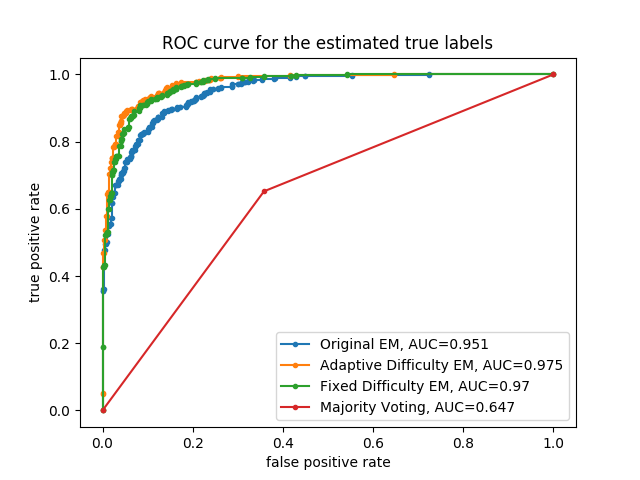
\includegraphics[width=5.0in]{image/roc_plot.png}
    \caption{ROC Curve for the estimated true labels. We compare our proposed methods with \textbf{Majority Voting} and \textbf{Original EM}} 
    \label{fig:gr}
\end{figure}

\textbf{2. Generalization of the learnt classifier}

From Table \ref{table:gt} we can see the generalization property of the learnt classifier is consistently well in all EM-based algorithms. Surprisingly, the proposed \textbf{Fixed Difficulty EM} algorithm increases the accuracy by a large margin but the AUC of it on the training set is inferior to \textbf{Adaptive Difficulty EM}. Our hypothesis is that the fixed imaged difficulty can play the role of regularization.

\begin{table}[H]
\caption{Guassian dataset: Accuracy of learnt classifier on test set}
\label{table:gt}
\begin{center}
\begin{tabular}{c c c c c }
		\toprule
		Method & Majority Voting & Original EM & Adaptive Difficulty EM & Fixed Difficulty EM	 \\
		\midrule
        Accuracy & $93.6 \pm 0.05$  & $94.00 \pm 0.11$ & $93.9 \pm 0.15$ & $\bm{94.4 \pm 0.13}$ \\
		\bottomrule
\end{tabular}
\end{center}
\end{table}

\textbf{3. Estimated expertise}

The actual sensitivity and specificity of each expert is marked as blue dots in Figure \ref{fig:ge}. We can see that the estimated expertise of our proposed EM algorithms is much closer to the actual values of sensitivity and specificity than the original EM algorithm. Moreover, we find that the estimated expertise of the two proposed algorithm is close. So different interpretations of image difficulty do not change the updating trajectory of experts' parameters much. We use $\alpha = \sigma (\frac{\bm{\lambda}^{1}}{4})$ and $\beta = \sigma(\frac{\bm{\lambda}^{2}}{4})$to recover the sensitivity and specificity of experts.

\begin{figure}[H]
    \centering
    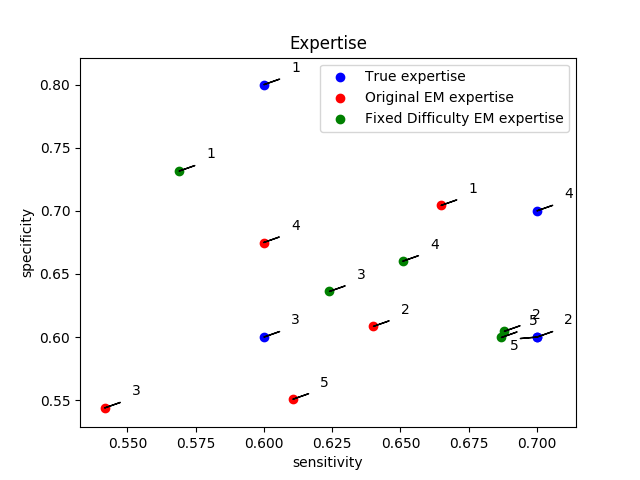
\includegraphics[width=5in]{image/expertise_g.png}
    \caption{Estimated Expertise on Gaussian dataset. The numbers denote corresponding experts. The expertise of \textbf{Adaptive Difficulty EM} and \textbf{Fixed Difficulty EM} is very close, so we only plot one of them. } 
    \label{fig:ge}
\end{figure}


\subsection{Dogs vs. Cats dataset}

In this experiments, the expert label real-world 2-class dataset. The experiment set up is almost the same as the two-dimension Gaussian mixture dataset except that the classifier used in this experiment is a four-layer convolutional neural network, and we use a pre-trained four-layer convolutional neural network to synthesis image difficulty, i.e the more uncertain the pretrained classifier is the more difficult this data point is.
We manually split the dataset into a $12,500$-image training set and a $12,500$-image test set to both test the accuracy of the estimated ground truth on the training set and the generalization performance of the learnt classifier on the test set.

\subsubsection{Structural Label}
Table \ref{table:dt}, Figure \ref{fig:dr} and Figure \ref{fig:de} summarize the results. The proposed \textbf{Fixed Difficulty EM} algorithm performs well both on estimating true labels and the generalization. The estimated expertise of \textbf{Original EM} marginally closer to the ground-truth expertise. 

We can see that \textbf{Majority Voting} can not converge in this case, and \textbf{Original EM} converges poorly. Actually, \textbf{Original EM} even can not converge in some experiments.


\begin{table}[htp]
\caption{Dogs vs. Cats dataset: Accuracy of learnt classifier on test set}
\label{table:dt}
\begin{center}
\begin{tabular}{c c c c c }
		\toprule
		Method & Majority Voting & Original EM & Adaptive Difficulty EM & Fixed Difficulty EM	 \\
		\midrule
        Accuracy & $50.0 \pm 0.0$  & $60.2 \pm 9.1$ & $70.4 \pm 0.9$ & $\bm{74.3 \pm 1.7}$ \\
		\bottomrule
\end{tabular}
\end{center}
\end{table}

\begin{figure}[htb]
    \centering
    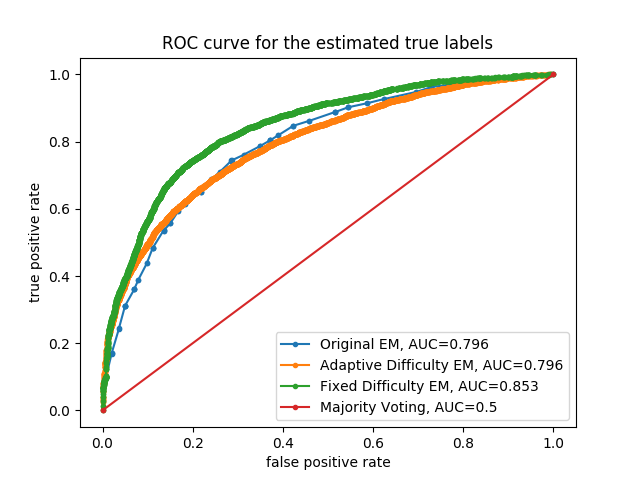
\includegraphics[width=5.5in]{image/roc_plot_dog.png}
    \caption{ROC Curve for the estimated true labels. We compare our proposed methods with \textbf{Majority Voting} and \textbf{Original EM}} 
    \label{fig:dr}
\end{figure}

\begin{figure}[htb]
    \centering
    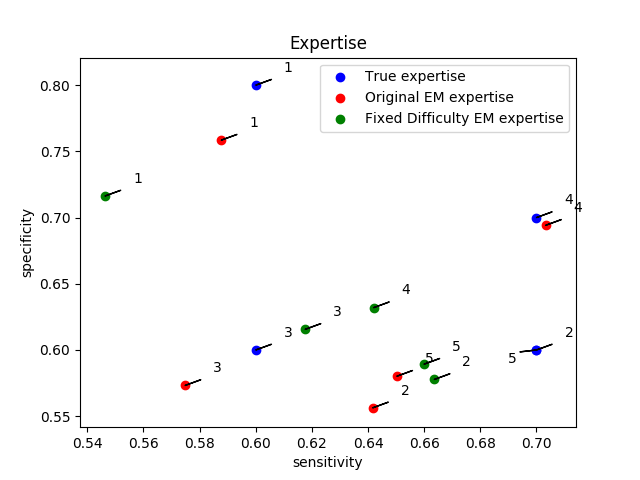
\includegraphics[width=5.5in]{image/expertise_dog.png}
    \caption{Estimated Expertise on Dogs vs Cats dataset. The numbers denote corresponding experts. The expertise of \textbf{Adaptive Difficulty EM} and \textbf{Fixed Difficulty EM} is very close, so we only plot one of them. } 
    \label{fig:de}
\end{figure}

\subsubsection{Non-structural Label}
Since in the experiments above, we use our assumption to synthesize the experts' labels, which is very structural. So we would like to compare these methods under settings that may be closer to real world, where the labels tend to be less structural. In such settings, with regard to every datapoint, an expert makes mistakes with probability $\frac{1}{3+k}$, where k is uniformly sampled from $\{0,1,2,3,4,5\}$. It should be noted that, to a single expert, the error probabilities corresponding to different images are also different. We only compare the generalization ability of the learnt classifier. The result is shown in Table \ref{table:rt}. The proposed algorithms still dominate other algorithms in this setting. The other two algorithms can not converge using non-structural labels.

\begin{table}[htp]
\caption{Non-structural label: Accuracy of learnt classifier on test set}
\label{table:rt}
\begin{center}
\begin{tabular}{c c c c c }
		\toprule
		Method & Majority Voting & Original EM & Adaptive Difficulty EM & Fixed Difficulty EM	 \\
		\midrule
        Accuracy & $50.0 \pm 0.0$  & $50.6 \pm 0.6$ & $76.7 \pm 0.8$ & $\bm{78.2 \pm 0.3}$ \\
		\bottomrule
\end{tabular}
\end{center}
\end{table}
\section{Discussions and Conclusion}


\section*{Acknowledgments}
Thanks Xiangyu Zhang for insightful discussions.
\section*{References}

\medskip

\small

[1] Barnes C, Shechtman E, Finkelstein A, et al. PatchMatch: A randomized correspondence algorithm for structural image editing[J]. ACM Transactions on Graphics (ToG), 2009, 28(3): 24.

\bibliography{ref}
\end{document}

